\documentclass[11pt]{standalone}

\usepackage{helvet}

\usepackage{ifthen}
\usepackage{tikz} 
\usetikzlibrary{shapes.misc}
\usetikzlibrary{arrows,arrows.meta}
\usetikzlibrary{calc,intersections, patterns, math}

\definecolor{pfeil}{RGB}{168,167,167}
\definecolor{petrol}{RGB}{0, 118, 136}
\definecolor{darkgoldenrod}{RGB}{184, 134, 11}
\colorlet{petrol-lighter}{petrol!40}
\colorlet{darkgoldenrod-lighter}{darkgoldenrod!40}

\begin{document}

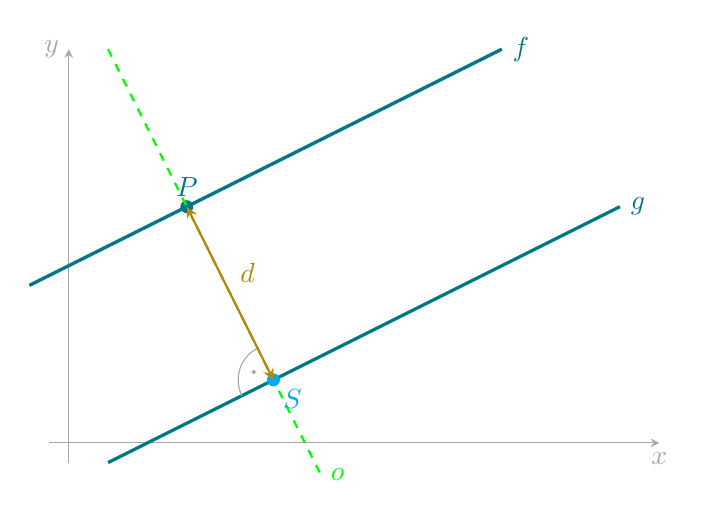
\begin{tikzpicture}[pfeil]

    % \draw[thick, fill=petrol!20, draw=petrol-lighter, rounded corners=2ex, opacity=0.5] (0,0) rectangle ++ (1.5,3.5);
    % \draw[thick, fill=darkgoldenrod!20, draw=darkgoldenrod-lighter, rounded corners=2ex, opacity=0.5] (5,0) rectangle ++ (1.5,3.5);

    \draw[-stealth] (-0.25,0) -- (7.5,0) node[below] {$x$};
    \draw[-stealth] (0,-0.25) -- (0,5)node[left]{$y$};



    \draw[petrol, fill] (1.5,3) circle (0.075) node[above] {$P$};

    \draw[petrol, very thick, domain=-0.5:5.5] plot(\x,{0.5*\x+2.25}) node[right] {$f$};

    \draw[petrol, very thick, domain=0.5:7] plot(\x,{0.5*\x-0.5}) node[right] {$g$};


    \draw[green, thick, dashed, domain=0.5:3.2] plot(\x,{-2*\x+6}) node[right] {$o$};

    \draw (2.2,0.6) arc(206.56:116.56:0.45);
    \draw[fill] (2.35,0.9) circle (0.02);

    \draw[cyan, fill] (2.6,0.8) circle (0.075) node[below right] {$S$};

    \draw[thick, darkgoldenrod, stealth-stealth] (1.5,3) -- node[above right] {$d$} (2.6,0.8);





    





\end{tikzpicture}

\end{document}
